\documentclass[conference]{IEEEtran}
\IEEEoverridecommandlockouts

\usepackage{cite}
\usepackage{amsmath,amssymb,amsfonts}
\usepackage{algorithmic}
\usepackage{graphicx}
\usepackage{textcomp}
\usepackage{xcolor}
\usepackage{booktabs}
\usepackage{url}

\def\BibTeX{{\rm B\kern-.05em{\sc i\kern-.025em b}\kern-.08em
    T\kern-.1667em\lower.7ex\hbox{E}\kern-.125emX}}

\begin{document}

\title{ROS\,2 Jazzy Environment Validation for an Autonomous Ackermann Vehicle:\\
Hardware and Simulation Platforms}

\author{
\IEEEauthorblockN{Andrew Abdelmalak}
\IEEEauthorblockA{\textit{Dept.\ of Mechatronics Engineering}\\
\textit{German University in Cairo}\\
Cairo, Egypt\\
andrew.abdelmalak@student.guc.edu.eg}
\and
\IEEEauthorblockN{Daniel Boules}
\IEEEauthorblockA{\textit{Dept.\ of Mechatronics Engineering}\\
\textit{German University in Cairo}\\
Cairo, Egypt\\
daniel.boules@student.guc.edu.eg}
\and
\IEEEauthorblockN{David Girgis}
\IEEEauthorblockA{\textit{Dept.\ of Mechatronics Engineering}\\
\textit{German University in Cairo}\\
Cairo, Egypt\\
david.girgis@student.guc.edu.eg}
\and
\IEEEauthorblockN{Kirolous Kirolous}
\IEEEauthorblockA{\textit{Dept.\ of Mechatronics Engineering}\\
\textit{German University in Cairo}\\
Cairo, Egypt\\
kirolous.kirolous@student.guc.edu.eg}
\and
\IEEEauthorblockN{Samir Yacoub}
\IEEEauthorblockA{\textit{Dept.\ of Mechatronics Engineering}\\
\textit{German University in Cairo}\\
Cairo, Egypt\\
samir.yacoub@student.guc.edu.eg}
\and
\IEEEauthorblockN{Youssef Salama}
\IEEEauthorblockA{\textit{Dept.\ of Mechatronics Engineering}\\
\textit{German University in Cairo}\\
Cairo, Egypt\\
youssef.salama@student.guc.edu.eg}
}

\maketitle

\begin{abstract}
Autonomous ground vehicles built on Ackermann steering geometry require a robust
software middleware layer before any perception, localization, or planning algorithms
can be developed. This paper documents the Milestone~1 validation of a ROS\,2 Jazzy
environment for an autonomous Ackermann vehicle project, targeting two distinct
execution contexts: an embedded Raspberry~Pi\,4 hardware platform and a desktop
Gazebo~Harmonic simulation platform. We describe the environment provisioning
procedure, the custom ROS\,2 Python packages developed for validation, and the
observable evidence---terminal logs and \texttt{ros2 doctor} diagnostics---confirming
correct operation. A publisher--subscriber node interacting with a simulated Ackermann
vehicle via \texttt{/cmd\_vel} and \texttt{/odom} topics is also presented. All five
\texttt{ros2 doctor} health checks passed on the hardware platform, and both
environments produced expected log output, confirming readiness for subsequent
milestones covering localization, navigation, and control.
\end{abstract}

\begin{IEEEkeywords}
ROS\,2, Jazzy, Ackermann steering, autonomous vehicle, Gazebo~Harmonic,
Raspberry~Pi, embedded robotics, validation
\end{IEEEkeywords}

% ============================================================
\section{Introduction}
\label{sec:intro}
% ============================================================

Autonomous wheeled vehicles pose a multi-disciplinary engineering challenge spanning
perception, localization, planning, and actuation. Modern robotics middleware---most
notably the Robot Operating System~2 (ROS\,2)---provides the publish-subscribe
communication fabric, hardware abstraction, and tooling necessary to integrate these
subsystems. Before any algorithm development can begin, however, the middleware
itself must be correctly installed, configured, and validated on every target platform.

This paper presents the complete Milestone~1 deliverables for Team~23 in the
MCTR1002 Autonomous Systems course at the German University in Cairo (GUC). The
goal is to provision and validate a ROS\,2 Jazzy environment on two platforms:
\begin{enumerate}
  \item A \emph{hardware} platform built around a Raspberry~Pi\,4 single-board
        computer running Ubuntu Noble~24.04;
  \item A \emph{simulation} platform pairing ROS\,2 Jazzy with Gazebo~Harmonic on
        a development laptop, providing a physics-simulated Ackermann vehicle model.
\end{enumerate}

Section~\ref{sec:related} reviews relevant literature on Ackermann vehicle autonomy.
Section~\ref{sec:arch} describes the overall system architecture.
Sections~\ref{sec:hw} and~\ref{sec:sim} detail the hardware and simulation
configurations, respectively.
Section~\ref{sec:results} presents validation results.
Section~\ref{sec:future} discusses limitations and future milestones.
Section~\ref{sec:conclusion} concludes.

% ============================================================
\section{Related Work}
\label{sec:related}
% ============================================================

An autonomous vehicle built around ROS\,2 sits at the intersection of four
well-studied research modules.

\subsection{System Architecture and Middleware}
ROS\,2 adopts a decentralized Data Distribution Service (DDS) communications
model that decouples high-level tasks (global path planning, SLAM) from
low-level controllers (motor drivers, servo actuators), enabling modular
development~\cite{Alkhareif2021}.

\subsection{Ackermann Steering Geometry and Kinematics}
The classic Ackermann constraint ensures all wheels roll on concentric circular
arcs, eliminating tire scrub. The geometric relation is
\begin{equation}
  \cot\delta_{o} - \cot\delta_{i} = \frac{T}{L},
  \label{eq:ackermann}
\end{equation}
where $\delta_{o}$ and $\delta_{i}$ are the outer and inner steering angles,
$T$ is the track width, and $L$ is the wheelbase~\cite{Chen2023}.

\subsection{Localization}
Extended Kalman Filters (EKF) formulated for Ackermann kinematics fuse wheel
encoder odometry with IMU data, yielding sub-centimetre positional accuracy when
implemented via the \texttt{robot\_localization} ROS\,2 package~\cite{Promkaew2024,Georgiev2025}.

\subsection{Navigation and Control}
Frenet-frame trajectory planning decouples longitudinal and lateral motion for
real-time operation in dynamic environments~\cite{Wang2020}. Model Predictive
Control (MPC) with explicit actuator-delay modelling outperforms classical Pure
Pursuit in path-tracking accuracy~\cite{Li2022}. Electronic differential control
via PID augmented with BP neural networks distributes drive torque across
Ackermann-steered axles~\cite{Zhang2022}.

% ============================================================
\section{System Architecture}
\label{sec:arch}
% ============================================================

The Milestone~1 architecture is deliberately minimal: it validates the
communication layer before introducing sensor data or planning algorithms.
Fig.~\ref{fig:arch} summarises the component layout.

\begin{figure}[htbp]
  \centering
  % Architecture diagram (text-based, no figure file needed)
  \fbox{\parbox{0.85\columnwidth}{\centering\small
    \textbf{Hardware Platform (RPi 4)}\\
    Ubuntu Noble 24.04 $\to$ ROS\,2 Jazzy (rmw\_fastrtps)\\
    \texttt{Validation\_Printing\_Node} @ 1\,Hz\\[4pt]
    \rule{0.7\columnwidth}{0.4pt}\\[4pt]
    \textbf{Simulation Platform (ASUS GA401QE)}\\
    Ubuntu + ROS\,2 Jazzy $\to$ Gazebo Harmonic\\
    Ackermann SUV model $\leftrightarrow$\\
    \texttt{Vehicle\_Pub\_Sub\_Node}
    (\texttt{/cmd\_vel} $\uparrow$, \texttt{/odom} $\downarrow$)
  }}
  \caption{Milestone~1 system architecture.}
  \label{fig:arch}
\end{figure}

The hardware and simulation platforms are developed in parallel. Both are
self-contained ROS\,2 computing nodes; cross-platform DDS discovery is not
required for Milestone~1.

% ============================================================
\section{Hardware Environment Setup and Validation}
\label{sec:hw}
% ============================================================

\subsection{Platform Specification}
The hardware platform is a Raspberry~Pi\,4~(4\,GB RAM) running Ubuntu
Noble~24.04~(ARM64). ROS\,2 Jazzy was installed via the official APT
repository (\texttt{ros-jazzy-desktop}) and sourced via
\texttt{/opt/ros/jazzy/setup.bash}.

\subsection{Environment Diagnostics}
The built-in \texttt{ros2 doctor} tool evaluates the ROS\,2 installation
across five health checks: network interface, RMW implementation, ROS\,2
packages, Python version, and middleware configuration. Table~\ref{tab:doctor}
reports the diagnostic results.

\begin{table}[htbp]
  \caption{ros2 doctor Diagnostic Results (Hardware Platform)}
  \label{tab:doctor}
  \centering
  \begin{tabular}{lc}
    \toprule
    Check & Status \\
    \midrule
    Network interface       & PASS \\
    RMW implementation      & PASS \\
    ROS\,2 package versions & PASS \\
    Python environment      & PASS \\
    Middleware configuration & PASS \\
    \midrule
    \textbf{Overall}        & \textbf{5/5 PASS} \\
    \bottomrule
  \end{tabular}
\end{table}

Running \texttt{ros2 doctor --report} confirmed:
distribution~=~\texttt{jazzy},
release~=~\texttt{6.8.0-1048-raspi},
middleware~=~\texttt{rmw\_fastrtps\_cpp}.
Fig.~\ref{fig:hw_ros2doctor} shows the terminal output.

\begin{figure}[htbp]
  \centering
  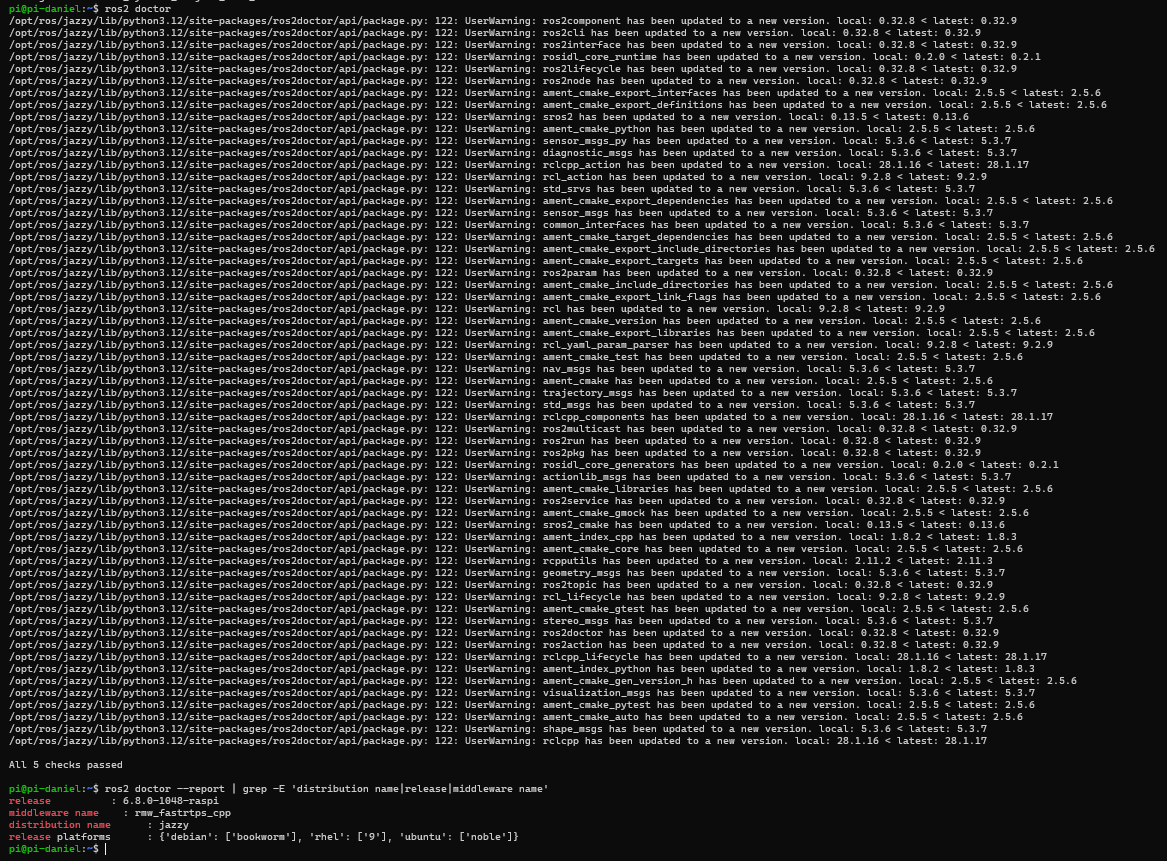
\includegraphics[width=\columnwidth]{figures/m1_hardware_ros2_doctor.png}
  \caption{Hardware platform: \texttt{ros2 doctor} reports all five checks
           passed on the Raspberry~Pi\,4.}
  \label{fig:hw_ros2doctor}
\end{figure}

\subsection{Validation Node}
A custom ROS\,2 Python node,
\texttt{Validation\_Printing\_Node\_Team\_23}, was authored within the
\texttt{Autonomous\_Systems\_Project\_Team\_23} package (ament\_python
build type). The node creates a 1\,Hz timer that logs the message:
\begin{quote}
  \textit{``ROS\,2 Jazzy is running successfully on Team~23 Raspberry~Pi''}
\end{quote}
Fig.~\ref{fig:hw_valnode} shows 26\,seconds of continuous operation on
the Raspberry~Pi\,4.

\begin{figure}[htbp]
  \centering
  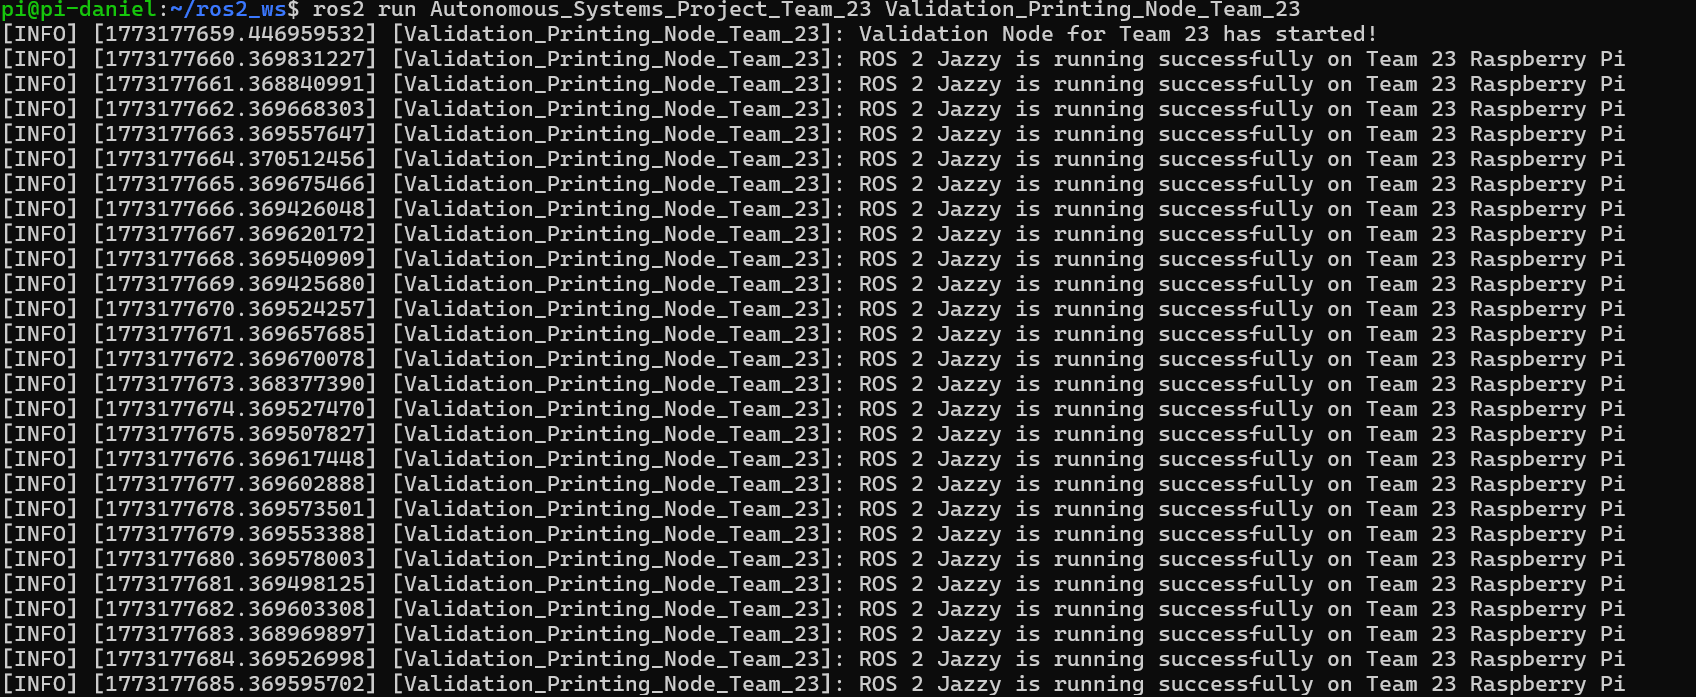
\includegraphics[width=\columnwidth]{figures/m1_hardware_validation_node.png}
  \caption{Hardware validation node executing at 1\,Hz: repeated confirmation
           messages observed over $\approx$26\,s of operation.}
  \label{fig:hw_valnode}
\end{figure}

% ============================================================
\section{Simulation Environment Setup and Validation}
\label{sec:sim}
% ============================================================

\subsection{Platform Specification}
The simulation platform is an ASUS ROG GA401QE laptop (AMD Ryzen~9~5900HX,
NVIDIA GTX~1650). ROS\,2 Jazzy and Gazebo~Harmonic were installed and
bridged via the \texttt{ros-jazzy-ros-gz} package.

\subsection{Ackermann Vehicle Model}
A SUV-type Ackermann-steered vehicle model was imported into Gazebo~Harmonic.
The ROS\,2--Gazebo bridge exposes the following topics (Table~\ref{tab:topics}).

\begin{table}[htbp]
  \caption{ROS\,2--Gazebo Bridge Topics (Simulation)}
  \label{tab:topics}
  \centering
  \small
  \begin{tabular}{lll}
    \toprule
    Topic & Message Type & Direction \\
    \midrule
    \texttt{/odom}              & Odometry          & Gazebo $\to$ ROS \\
    \texttt{/scan}              & LaserScan         & Gazebo $\to$ ROS \\
    \texttt{/camera/image\_raw} & Image             & Gazebo $\to$ ROS \\
    \texttt{/tf}                & TFMessage         & Gazebo $\to$ ROS \\
    \texttt{/cmd\_vel}          & Twist             & ROS $\to$ Gazebo \\
    \texttt{/ackermann\_cmd}    & AckermannDriveStamped & ROS $\to$ Gazebo \\
    \bottomrule
  \end{tabular}
\end{table}

\subsection{Publisher--Subscriber Node}
The \texttt{Vehicle\_Pub\_Sub\_Node\_Team\_23} node publishes a constant
velocity command (\texttt{linear.x}~$= 0.5$\,m/s,
\texttt{angular.z}~$= 0.2$\,rad/s) to \texttt{/cmd\_vel} at 1\,Hz and
subscribes to \texttt{/odom} to confirm pose feedback, closing the first
software control loop in simulation.

\subsection{Validation Node}
A simulation-side validation node, \texttt{validation\_printing\_node}, was
executed using the \texttt{ros2 daemon} to initialise DDS discovery. The node
logged a single confirmation message and exited cleanly.
Fig.~\ref{fig:sim_valnode} shows the terminal output on the simulation laptop.

\begin{figure}[htbp]
  \centering
  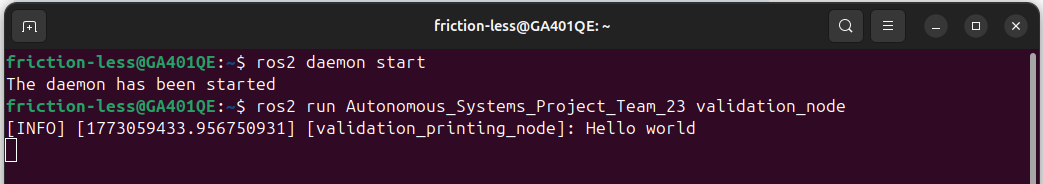
\includegraphics[width=\columnwidth]{figures/m1_simulation_validation_node.png}
  \caption{Simulation environment: ROS\,2 daemon started and validation node
           confirms ROS\,2 Jazzy operation on the development laptop.}
  \label{fig:sim_valnode}
\end{figure}

% ============================================================
\section{Results}
\label{sec:results}
% ============================================================

Table~\ref{tab:results} summarises all Milestone~1 success criteria and their
achieved status.

\begin{table}[htbp]
  \caption{Milestone~1 Validation Summary}
  \label{tab:results}
  \centering
  \small
  \begin{tabular}{lcc}
    \toprule
    Deliverable & Platform & Status \\
    \midrule
    ROS\,2 Jazzy installation         & Hardware  & \checkmark \\
    ros2 doctor (5/5 checks)          & Hardware  & \checkmark \\
    Validation node @ 1\,Hz           & Hardware  & \checkmark \\
    ROS\,2 Jazzy installation         & Simulation & \checkmark \\
    Simulation validation node        & Simulation & \checkmark \\
    Ackermann vehicle in Gazebo       & Simulation & \checkmark \\
    Publisher--subscriber (/cmd\_vel, /odom) & Simulation & \checkmark \\
    \bottomrule
  \end{tabular}
\end{table}

All seven deliverables were achieved. The hardware environment ran
\texttt{ros2 doctor} with a perfect five-of-five diagnostic score, confirming
the ROS\,2~Jazzy DDS communication stack is correctly configured.
The simulation environment demonstrated bidirectional topic communication
between a ROS\,2 Python node and a Gazebo~Harmonic Ackermann vehicle model,
providing the foundation for subsequent milestones.

% ============================================================
\section{Limitations and Future Work}
\label{sec:future}
% ============================================================

Milestone~1 is limited to environment validation. The following items remain
for subsequent milestones:

\begin{itemize}
  \item \textbf{Localization}: integrate wheel-encoder odometry with IMU data
        via EKF (\texttt{robot\_localization} package) following
        \cite{Promkaew2024,Georgiev2025}.
  \item \textbf{Perception}: activate \texttt{/scan} (LiDAR) and
        \texttt{/camera/image\_raw} topic pipelines for obstacle detection.
  \item \textbf{Navigation}: implement Frenet-frame trajectory planning
        \cite{Wang2020} and an MPC local planner \cite{Li2022}.
  \item \textbf{Control}: realise Ackermann-correct steering geometry
        per~\eqref{eq:ackermann} in the physical actuator layer.
    \item \textbf{Package cleanup}: align hardware/simulation package metadata
      (description, maintainer, license) and keep explicit ROS dependency
      declarations synchronized with imported interfaces.
\end{itemize}

% ============================================================
\section{Conclusion}
\label{sec:conclusion}
% ============================================================

This paper presented the complete ROS\,2 Jazzy environment validation for
Team~23's autonomous Ackermann vehicle project (Milestone~1, MCTR1002 at GUC).
The Raspberry~Pi\,4 hardware platform passed all five \texttt{ros2 doctor}
diagnostics and ran a 1\,Hz validation node for over 26\,seconds. The Gazebo
Harmonic simulation platform instantiated a full Ackermann SUV model with six
ROS\,2 topics and executed a publisher--subscriber node commanding and reading
pose from the simulated vehicle. These validated environments constitute the
communication backbone on which perception, localization, and motion-planning
layers will be built in forthcoming milestones.

\bibliographystyle{IEEEtran}
\bibliography{references}

\end{document}
